\chapter{Risultati}
\label{cap:risultati}

\textit{\indent Questo capitolo presenta un'analisi dettagliata dei risultati ottenuti dagli esperimenti descritti nel capitolo precedente e una riflessione su di essi.}

\section{Risultati degli Esperimenti QUIC}
\subsection{Risultati Esperimento 1}
In questa sezione si analizzano i risultati ottenuti dall'esperimento in cui abbiamo simulato un \emph{server web QUIC} con un comportamento modificato. 
Il \emph{server} è configurato per operare come se non ricevesse mai conferme dei pacchetti inviati, mantenendo al contempo un \emph{PTO} impostato a 0. 
Di seguito, vengono presentati i risultati emersi accompagnati dai relativi grafici. I dati in versione tabellare sono presenti nell'Appendice.
\\\\
Le modifiche apportate al \emph{server} hanno prodotto risultati decisamente diversi rispetto alla connessione normale. 
In condizioni standard, la trasmissione ha generato un traffico di circa 5.8 \emph{Mb} con un totale di circa 4100 pacchetti scambiati. 
Questi dati rappresentano il punto di riferimento per valutare l'impatto dei cambiamenti al comportamento del \emph{server}.
\\\\
Come illustrato in Figura \ref{grafico12}, che mostra il confronto del consumo dati tra i vari esperimenti e lo scenario standard, le modifiche hanno prodotto effetti notevolmente diversi.
Negli scenari di \emph{Retransmission 1 e 2}, si è osservato un incremento del traffico dati di più del $200\%$, passando dai 5.8 \emph{Mb} dello scenario standard a circa 13 \emph{Mb} nel primo caso e 15 \emph{Mb} nel secondo. 
Parallelamente, come viene evidenziato in Figura \ref{grafico2}, il numero di pacchetti scambiati è aumentato da 4100 a circa 18000. 
Tuttavia, questi scenari hanno presentato problemi di congestione e latenza che ne hanno compromesso l'applicabilità pratica.
\\\\
Le varianti 4 e 5 hanno mostrato un comportamento differente, principalmente grazie alla modifica che permette l'accettazione di un \emph{ACK} ogni due ricevuti.
La variante 4, che non ignora la richiesta di chiusura della connessione, ha registrato un consumo di 58 \emph{Mb} e circa 65000 pacchetti, senza causare latenza o congestioni. 
La variante 5, che invece blocca le richieste di chiusura della connessione, ha mostrato un consumo di 29 \emph{Mb} e circa 35000 pacchetti, manifestando una latenza minima nel caricamento dei contenuti.
\begin{figure}[h!]
    \centering
    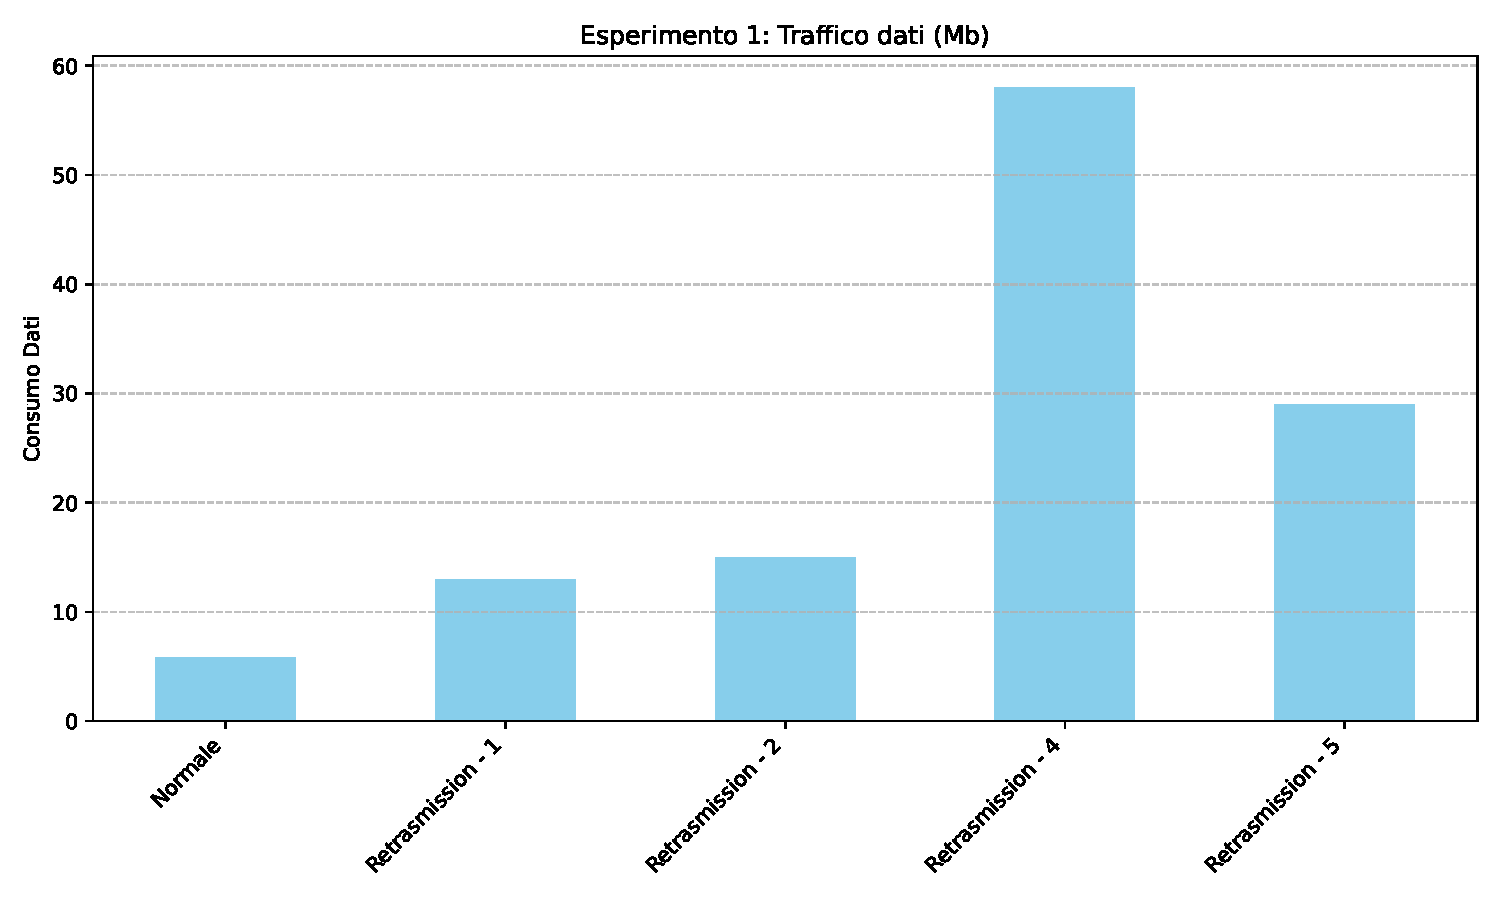
\includegraphics[width=\textwidth]{graphTraffico1.pdf}
    \caption{Traffico Dati (Mb)}
    \subcaption{da fare}
    \label{grafico12}
\end{figure}

\begin{figure}[h!]
    \centering
    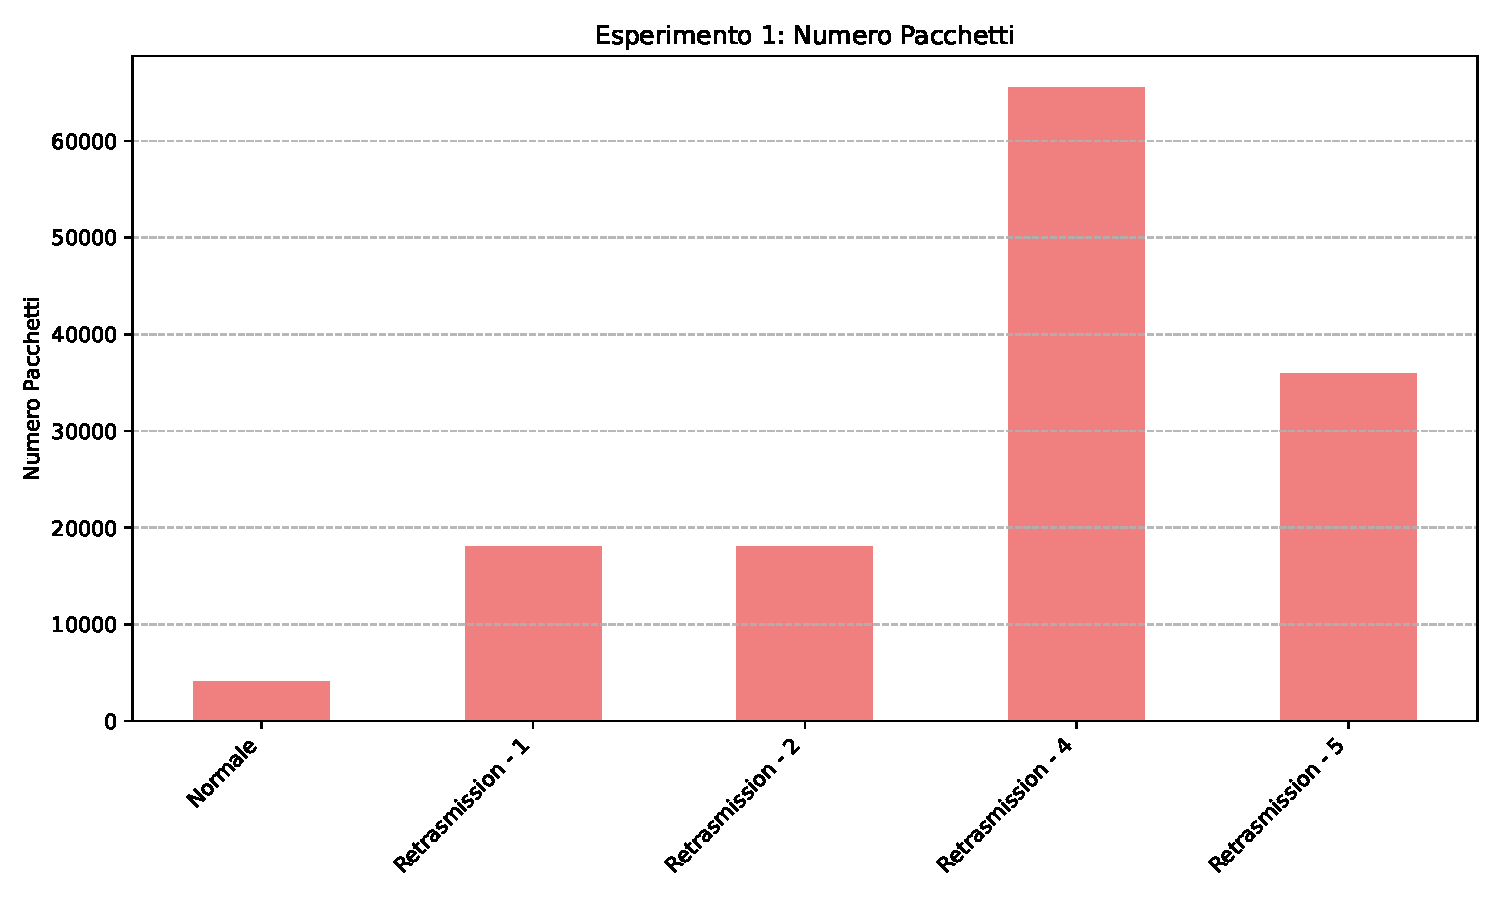
\includegraphics[width=\textwidth]{graphNumPacchetti1.pdf}
    \caption{Numero Pacchetti}
    \subcaption{da fare}
    \label{grafico1}
\end{figure}

\noindent Questi risultati evidenziano come la gestione degli \emph{ACK} unita ad un \emph{PTO} costante a 0 influenzi significativamente sia il consumo di dati che il numero di pacchetti scambiati.
La variante 4, che aumenta tot e tot e non comporta latenza o congestione. Significa tot e tot aumentando il traffico contabilizzato di un possibile utente. 
\subsection{Risultati Esperimento 2}
\begin{figure}[h!]
    \centering
    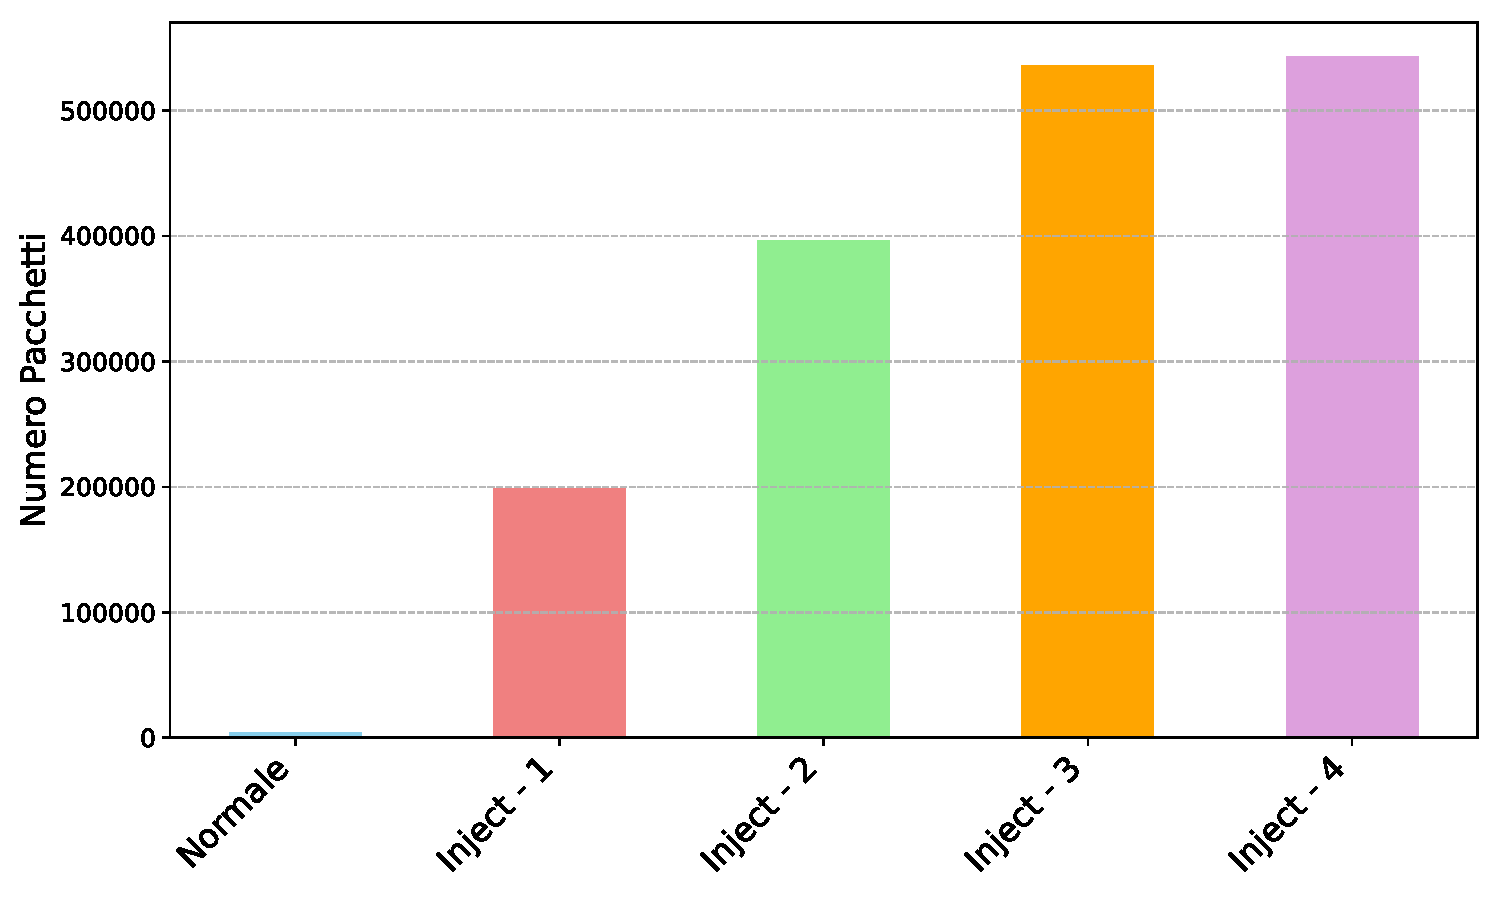
\includegraphics[width=\textwidth]{graphNumPacchetti2.pdf}
    \caption{Descrizione del grafico}
    \label{grafico2}
\end{figure}
\begin{figure}[h!]
    \centering
    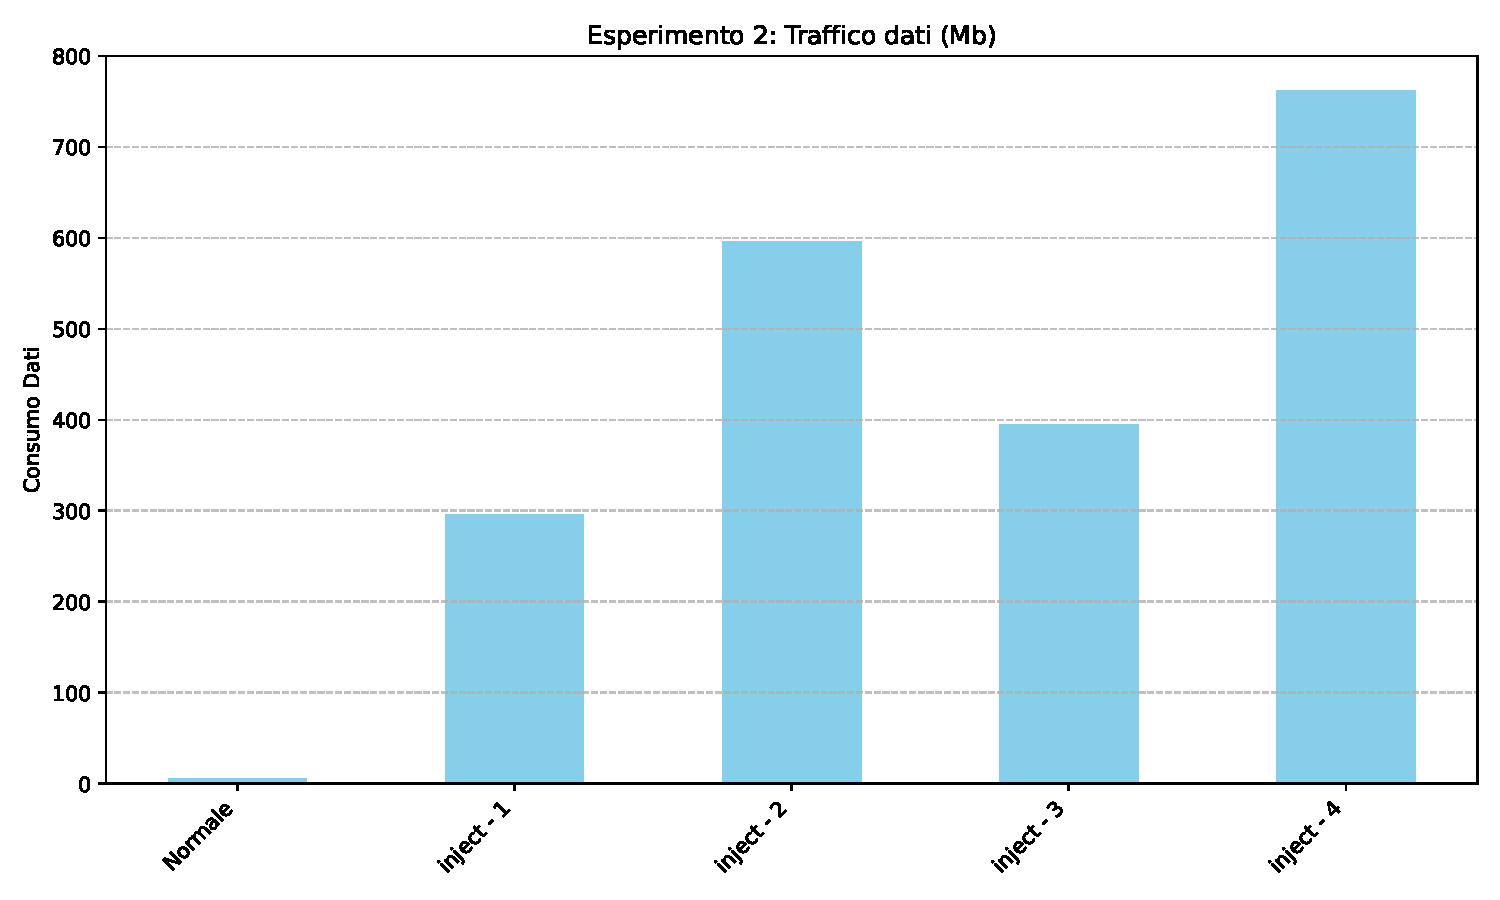
\includegraphics[width=\textwidth]{graphTraffico2.pdf}
    \caption{Descrizione del grafico}
    \label{grafico22}
\end{figure}
\begin{figure}[h!]
    \centering
    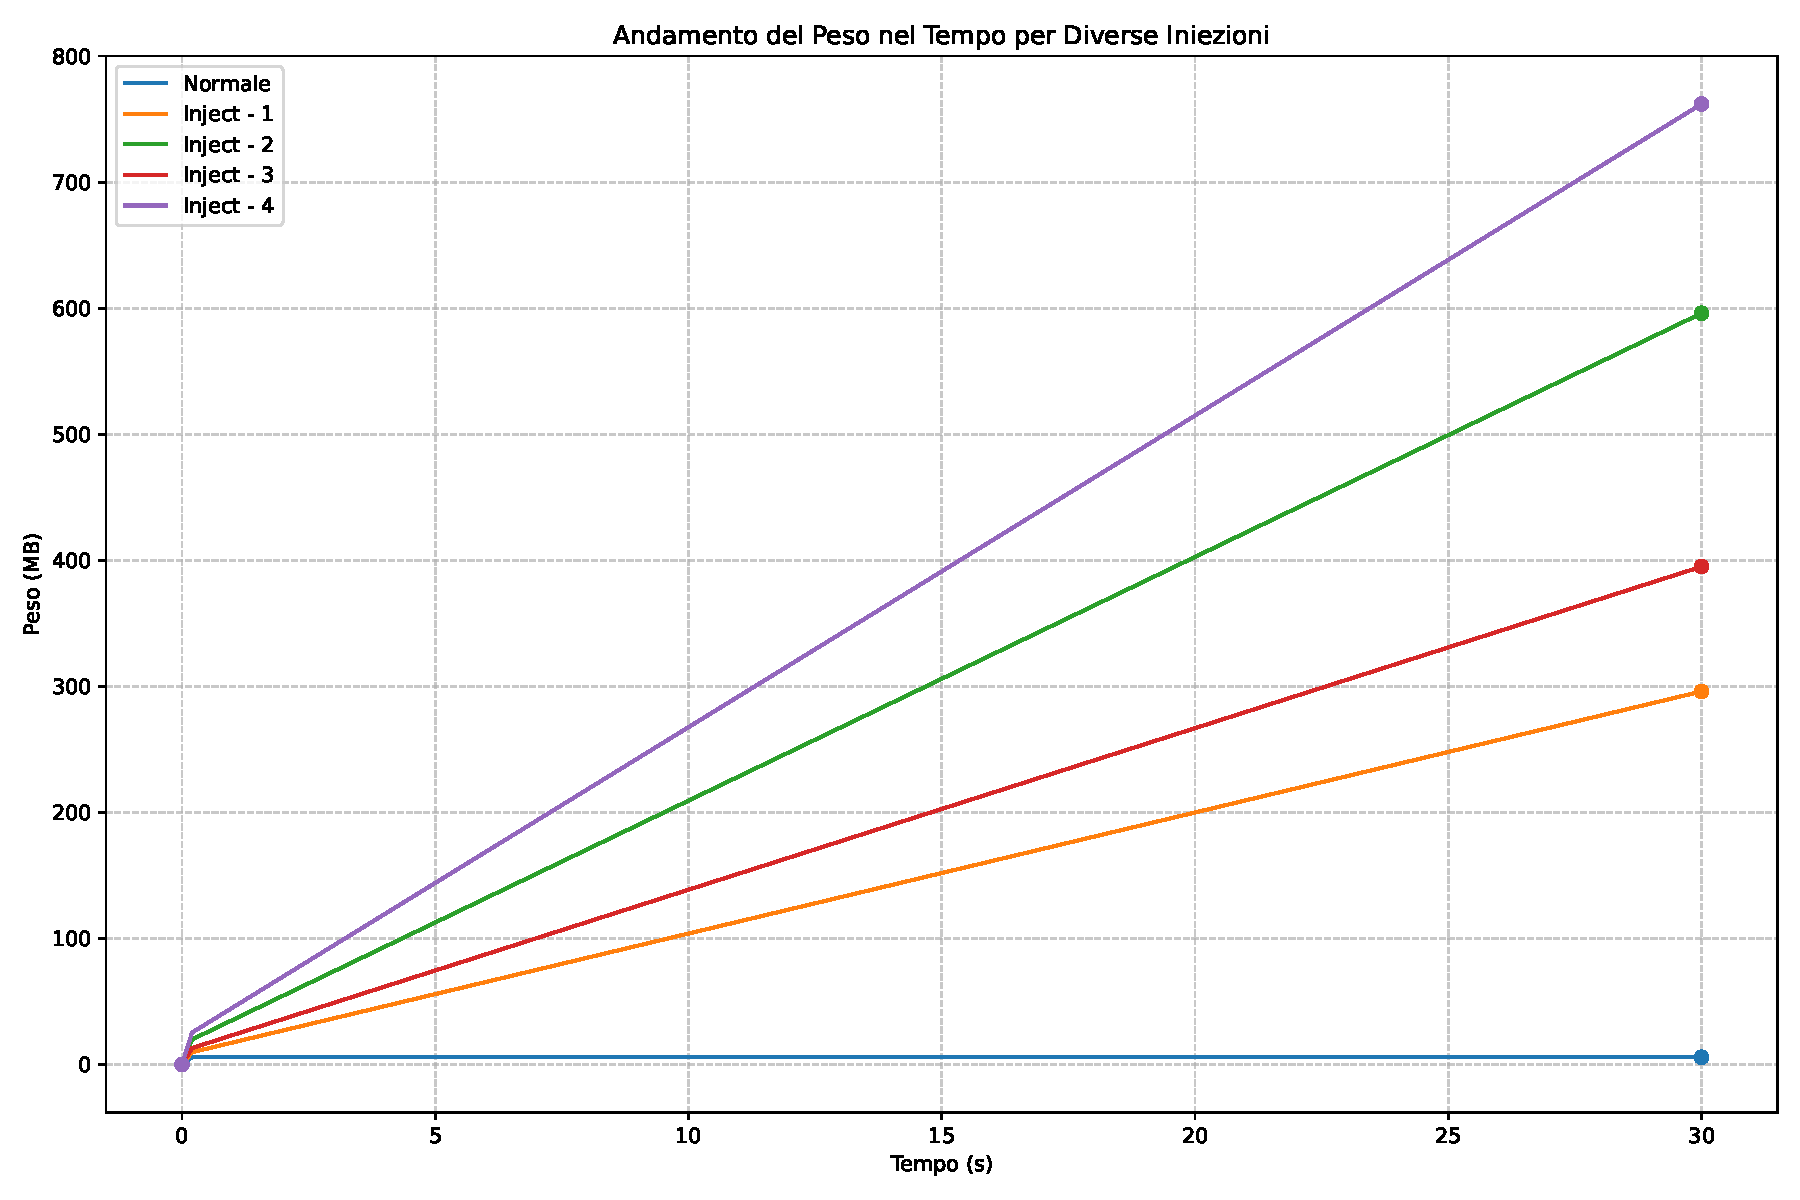
\includegraphics[width=\textwidth]{graphTrafficoTempo.pdf}
    \caption{Descrizione del grafico}
    \label{grafico23}
\end{figure}
\subsection{Risultati Esperimento 3}
\begin{figure}[h!]
    \centering
    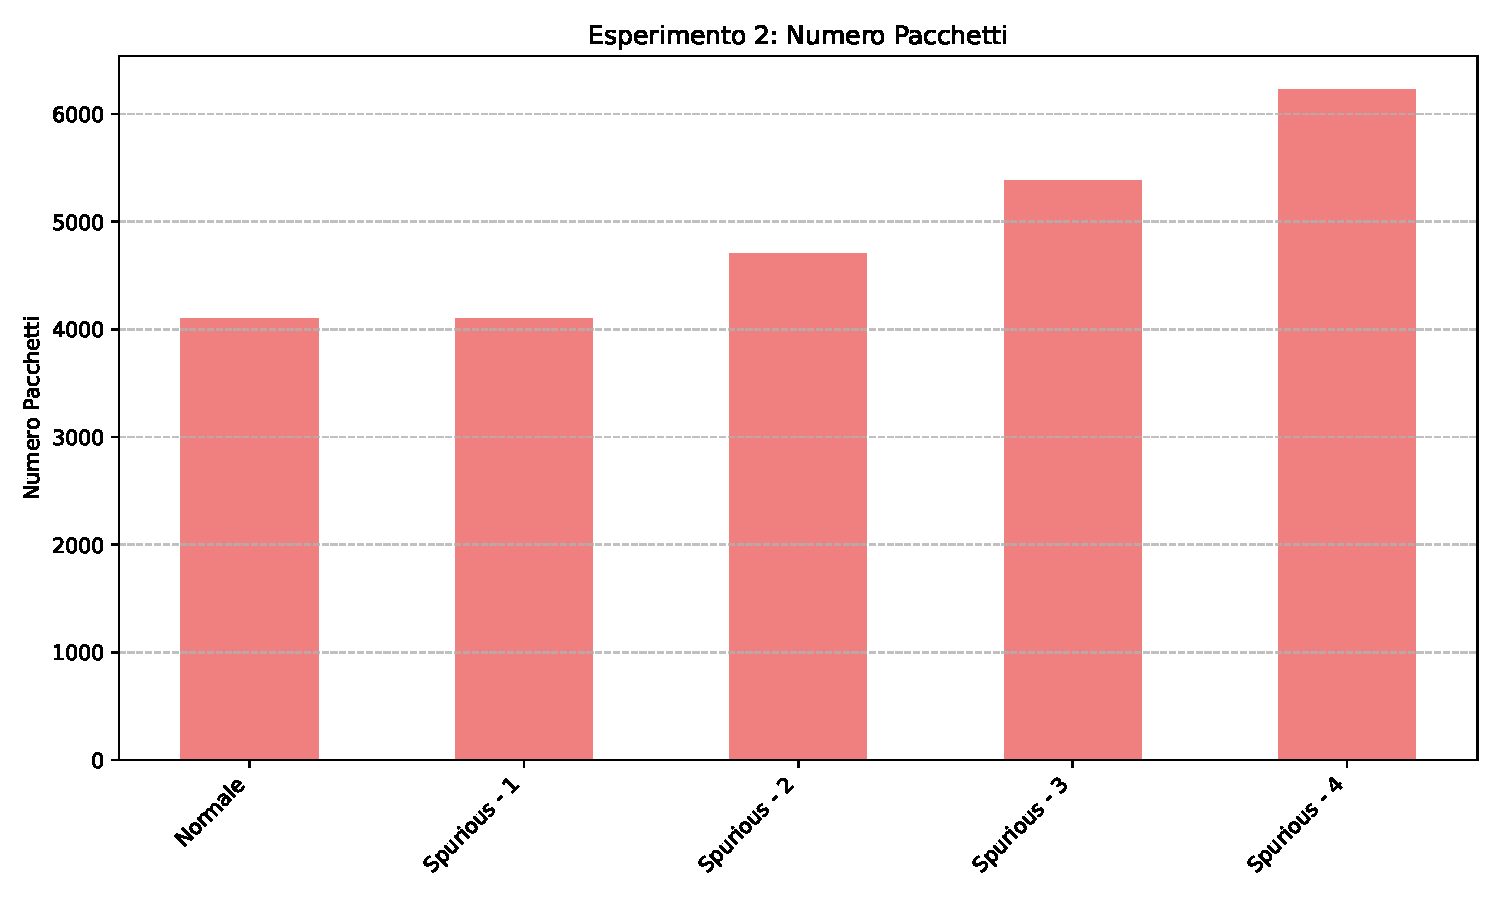
\includegraphics[width=\textwidth]{graphNumPacchetti3.pdf}
    \caption{Descrizione del grafico}
    \label{grafico3}
\end{figure}
\begin{figure}[h!]
    \centering
    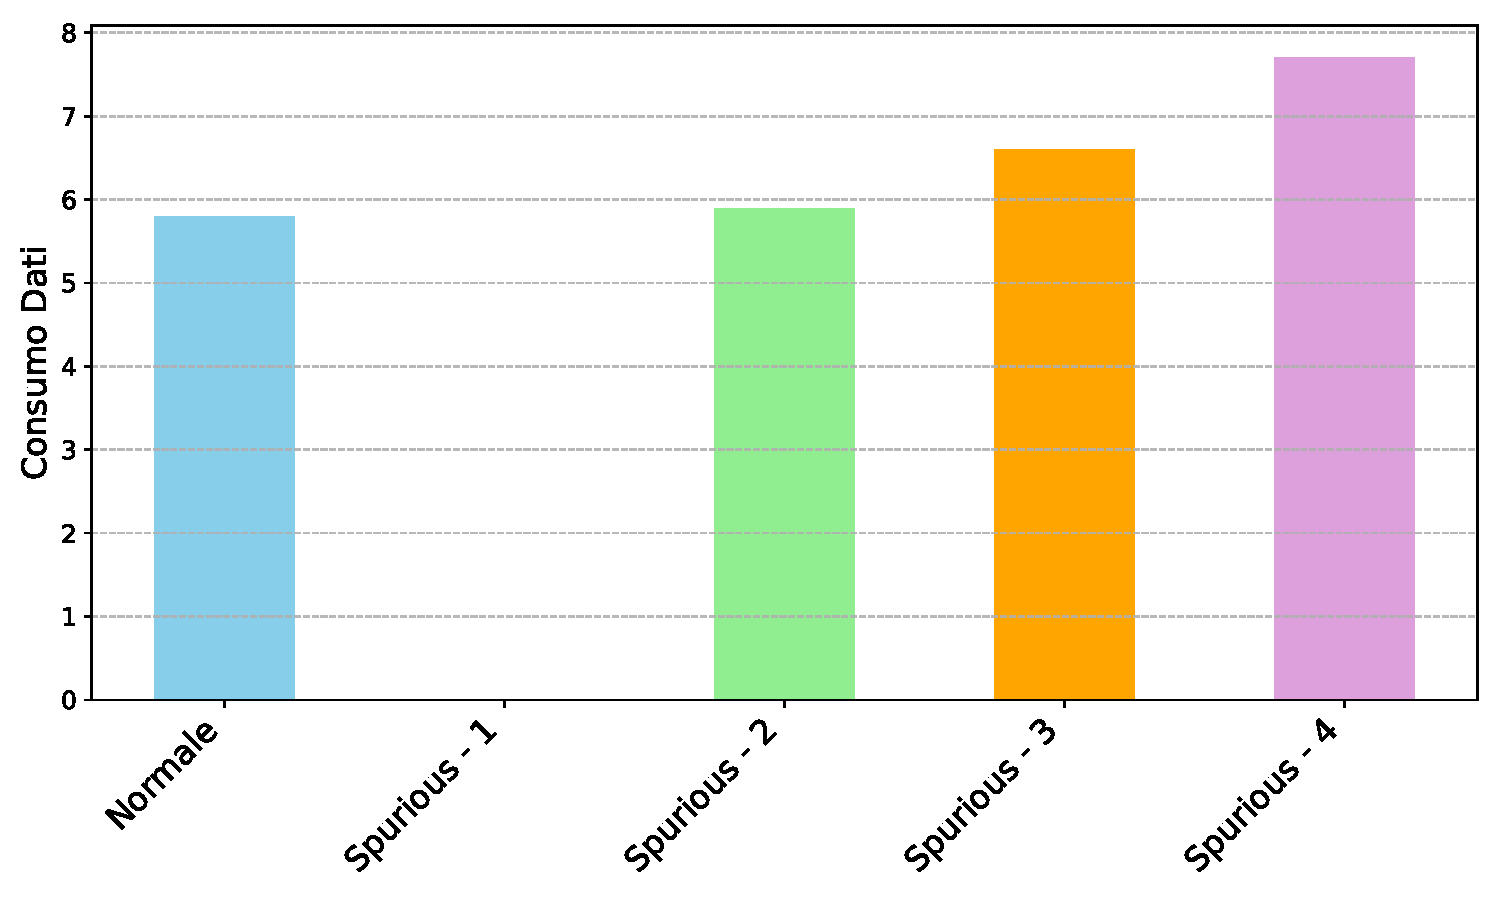
\includegraphics[width=\textwidth]{graphTraffico3.pdf}
    \caption{Descrizione del grafico}
    \label{grafico32}
\end{figure}
